\chapter{А так звучит красиво? Гармоничность}
\label{ch:harmony}


\section{Сколько вешать в полутонах? Интервалы}
\label{ch:harmony:interval}

\begin{Definition}[Интервал]
    \emph{Интервал} --- это расстояние между \emph{двумя} музыкальными звуками, выраженное в полутонах. 
\end{Definition}

Это определение для математиков. Для музыкантов же интервалы \emph{звучат}! Если два звука прозвучали одновременно, то интервал называется \emph{гармоническим}, а если друг за другом --- \emph{мелодическим}.

\begin{Example}[Послушаем гармонические интервалы]
    \label{ex:harmony:interval:string5and6}
    Возьмите настроенную гитару. Поиграем на 5 и 6-й струне. Если гитара настроена страндартно, то 6-я струна на 5-м ладу прозвучит в унисон с открытой 5-й струной. Такое расстояние в 0 полутонов музыканты называют \emph{примой}. 
    
    Инструмент обязательно должен быть настроен! Иначе эксперимент не получится.
    
    Теперь расслабьтесь, успокойтесь, забудьте обо всех горестях и радостях. Сосредоточьтесь на своем дыхании. Существует только ваше дыхание. Абсолютный покой. 
    
    Не получается? Чёрт с ним!

    Вам нужно будет оценить свои ощущения от сыгранных интервалов. Поставьте каждому интервалу оценку, например по 5-и балльной шкале: 1(ужос), 2(срам), 3(терпимо), 4(хорошо), 5(прекрасно).
    
    Начнем. Зажимите 6-ю струну на 5-м ладу и одновременно сыграйте две струны: 6-ю и 5-ю. Звучит гармонический интервал \emph{прима}! Интервал в ноль полутонов. Прислушиваемся к ощущениям, ставим приме оценку.
    
    Продолжаем оценивать интервалы. Играем одновременно 5-ю открытую струну и 6-ю струну на 6-м ладу. Расстояние в 1 полутон. Оценивайте результат.
    
    И так далее, играем интервал в 2 полутона (6-я струна на 7-м ладу) и так далее до интервала в 12 полутонов (6-я струна на 17 ладу). 
    
    Читая этот раздел, периодически поглядывайте на свои записи. Будет полезно.
\end{Example}

Приятный на слух интервал (неважно, гармонический или мелодический) музыканты называют \emph{консонансом}, а неприятный --- \emph{диссонансом}. 

Чтобы глубже разобраться в том, почему звучание одного интервала нам нравится, а другого --- нет, визуализируем результат наложения двух звуков. Пусть функция $\sin(x)$ изображает основной тон исходного звука. Функция $\sin(x\cdot(\sqrt[12]{2})^n)$ будет изображать звук, который \emph{выше} исходного на $n$ \emph{полутонов}. Результату совместного звучания (то есть гармоническому интервалу) будет соответствовать их сумма\footnote{В Интернете масса сайтов, позволяющих построить график функции. Более того, просто вбейте в гугл \texttt{sin(x)+sin(x*(2\^{}(1/12)))} и дивитесь чудесам Технологии!}:

\begin{equation}
    \label{eq:harmony:interval:sin}
    \sin(x) + \sin(x\cdot(\sqrt[12]{2})^n).
\end{equation}

Результаты построения графиков совместного звучания (построен красным цветом) на фоне исходного звука (синий цвет) для интервалов от $n=1$ до $n=11$ полутонов (т.е. в рамках октавы) приведены в таблицах \ref{t:harmony:interval:disso-1-2-10-11}, \ref{t:harmony:interval:conso-3-4-8-9}, \ref{t:harmony:interval:conso-5-7}, \ref{t:harmony:interval:disso-6}.

Диссонансы приведены в таблицах \ref{t:harmony:interval:disso-1-2-10-11} и \ref{t:harmony:interval:disso-6}. Диссонансы получаются на интервалах в 1,2,6,10 или 11 полутонов. Значит вам не должны были понравиться интервалы на 6,7,11,15,16 ладах 6-й струны, если вы обратили внимание на пример \ref{ex:harmony:interval:string5and6}. Только не говорите, что понравились! Пора сходить к доктору!!! Не затягивайте. 

\begin{table}[!ht]
    \caption{Диссонансы в графиках функции \eqref{eq:harmony:interval:sin}}
    \label{t:harmony:interval:disso-1-2-10-11}
    \centering
    \begin{tabular}{c|c}
        \hline\hline
        1 полутон, $n=1$        & 2 полутона, $n=2$ \\
        малая секунда           & большая секунда \\
        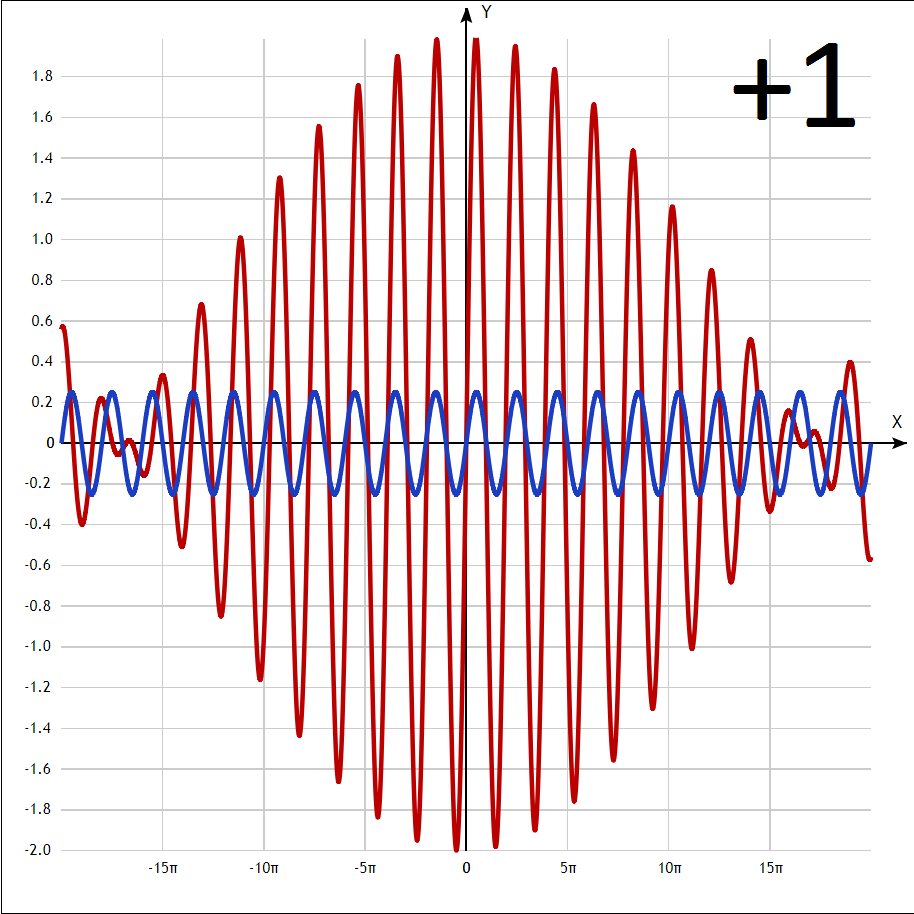
\includegraphics[width=0.45\textwidth]{fig/intervals/i01}
            & 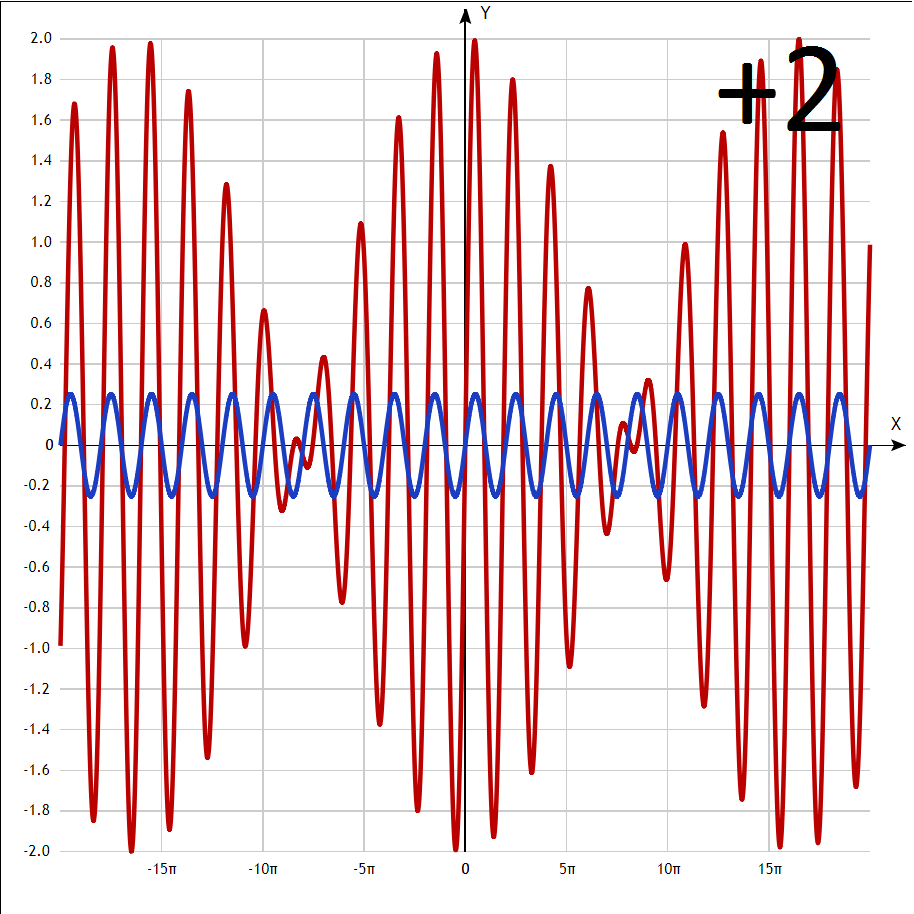
\includegraphics[width=0.45\textwidth]{fig/intervals/i02} \\
        \hline\hline
        10 полутонов, $n=10$    & 11 полутонов, $n=11$ \\
        малая септима           & большая септима \\
        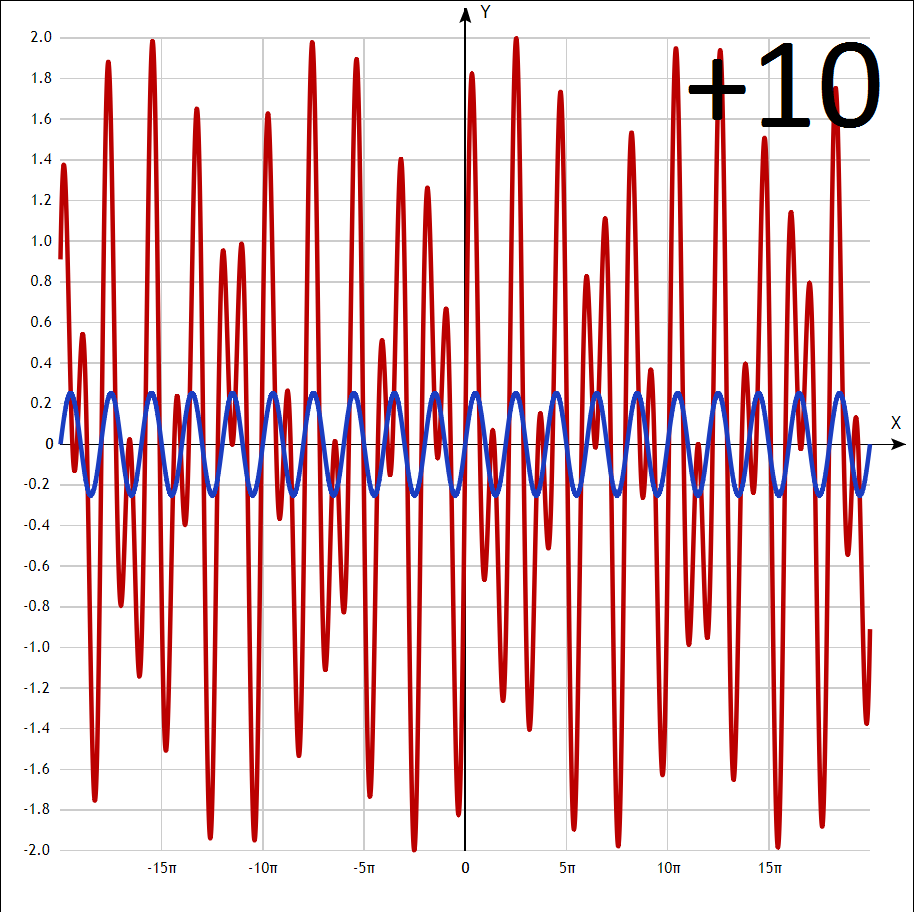
\includegraphics[width=0.45\textwidth]{fig/intervals/i10}
            & 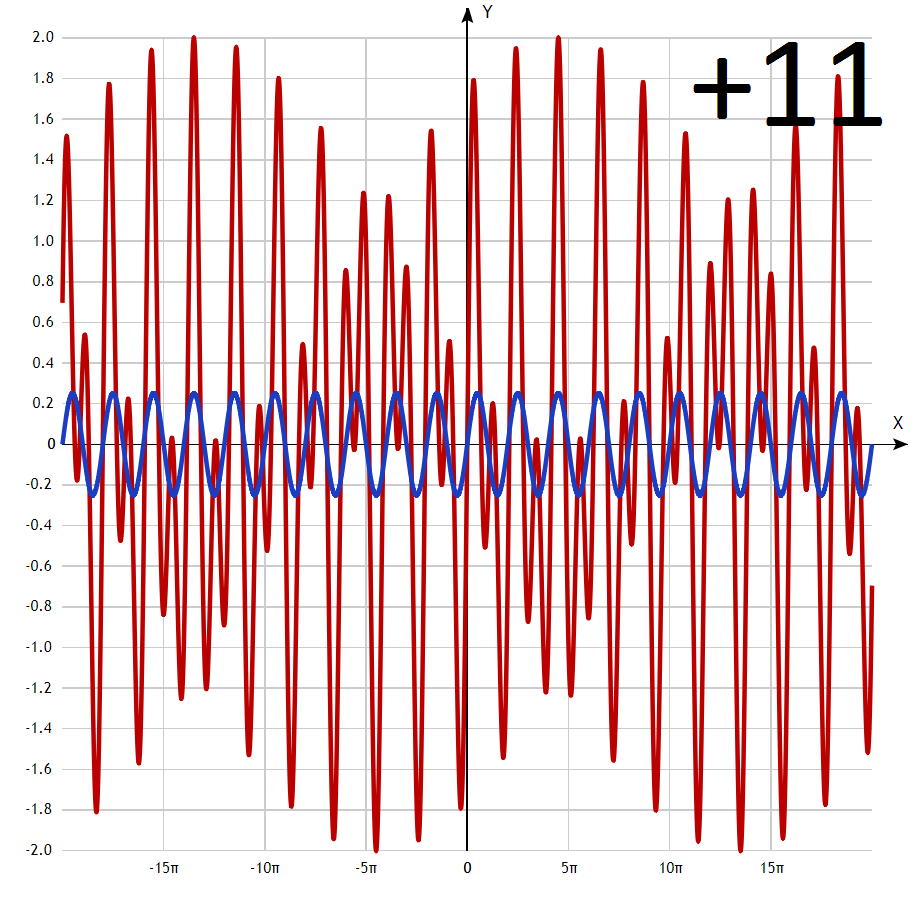
\includegraphics[width=0.45\textwidth]{fig/intervals/i11} \\
        \hline\hline
    \end{tabular}
\end{table}

Приглядитесь к приведенным графикам и попробуйте самостоятельно сделать выводы о причинах благозвучия консонансов и некоей хаотичности диссонансов. Консонансы, кстати, принято разделять на:
\begin{itemize}
    \item \emph{абсолютные}. Это полностью сливающиеся на слух интервалы в 0 полутонов (\emph{прима}, если помните) или кратные 12-ти полутонам. О причинах слияния этих звуков мы поговорили в самом начале, см. раздел \ref{ch:music:tone}. Интервал в 12 полутонов называется \emph{октавой}.
    
    \item \emph{совершенные}. Расстояние между звуками составляет 5 или 7 полутонов. См. таблицу \ref{t:harmony:interval:conso-5-7}. Смело можете понизить или повысить любой из звуков такого интервала на одну или несколько октав (12 полутонов) и совершенный консонанс останется\footnote{Уже заметили, что 5+7=12?}. Эти интервалы не сливаются на слух, но звучат благозвучно. Отличник среди консонансов.
    
    \item \emph{несовершенные}. Звуки не сливаются, точно не диссонанс, но и не совершенный консонанс. Короче, консонанс с помарочкой. Когда мы слышим несовершенный консонанс, то хочется, чтобы он побыстрее перешел консонанс совершенный, стал отличником. Разница между звуками составляет 3, 4, 8 или 9 полутонов. Точно так же, любой звук такого интервала можно понизить или повысить на октаву и несовершенство останется.
\end{itemize}


\begin{table}[!ht]
    \caption{Несовершенные консонансы в графиках функции \eqref{eq:harmony:interval:sin}}
    \label{t:harmony:interval:conso-3-4-8-9}
    \centering
    \begin{tabular}{c|c}
        \hline\hline
        3 полутона, $n=3$   & 4 полутона, $n=4$ \\
        малая терция        & большая терция \\
        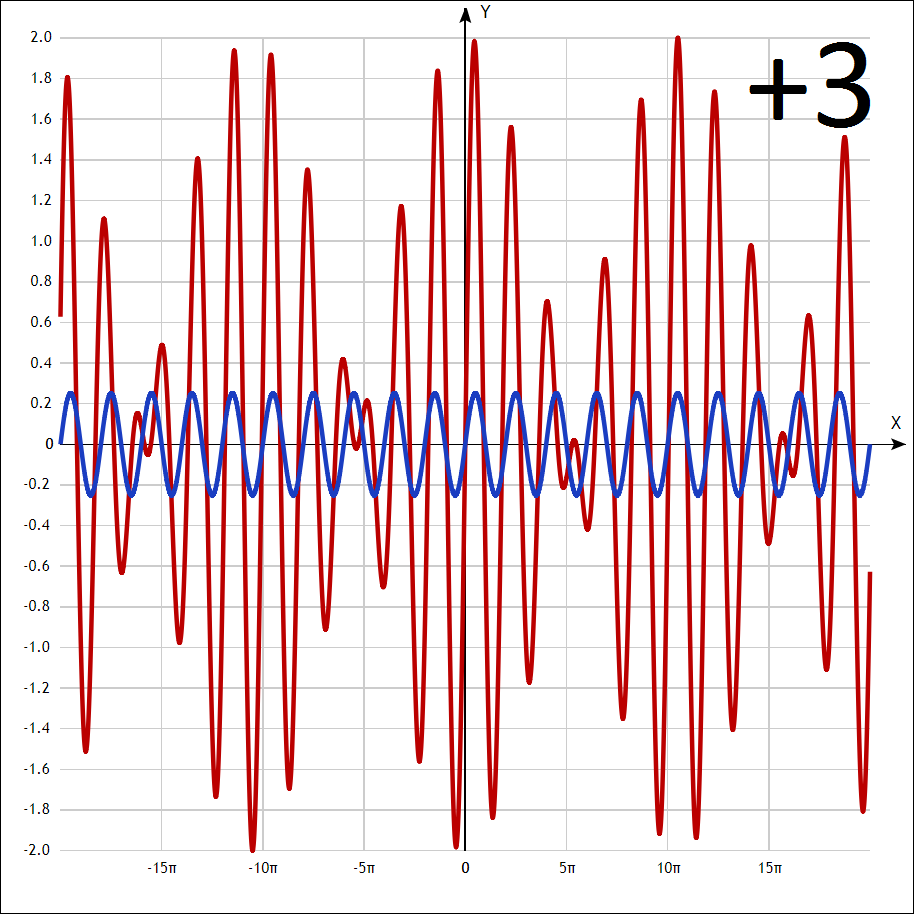
\includegraphics[width=0.45\textwidth]{fig/intervals/i03}
            & 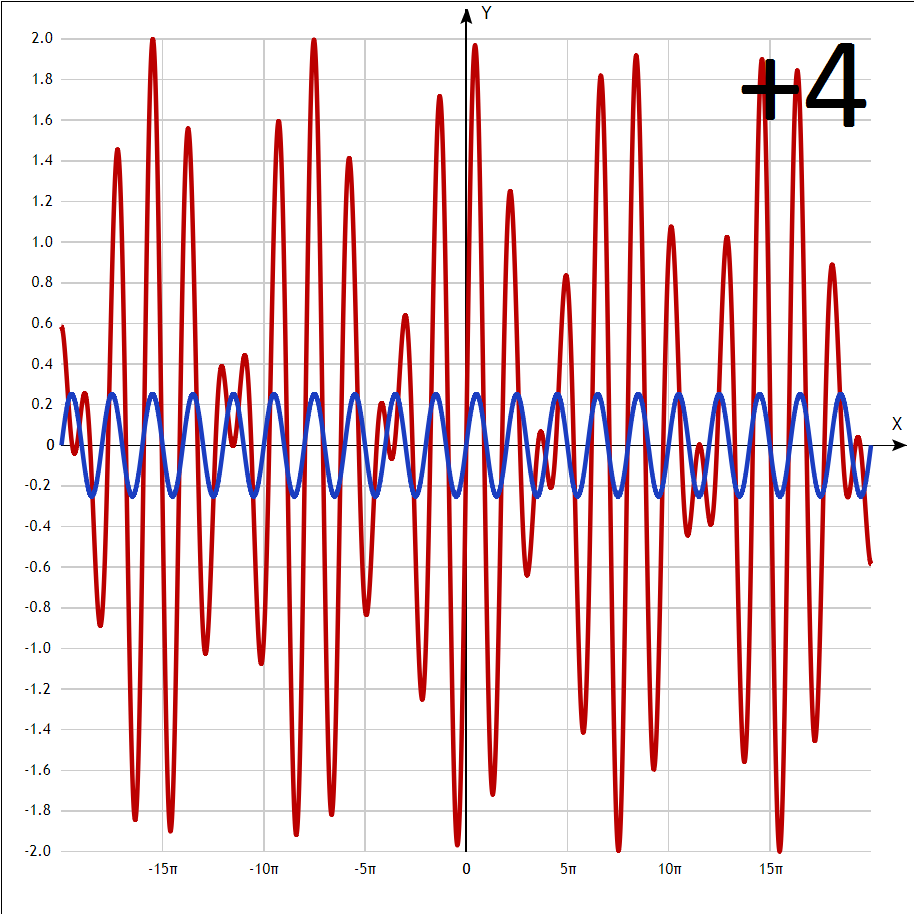
\includegraphics[width=0.45\textwidth]{fig/intervals/i04} \\
        \hline\hline
        8 полутонов, $n=8$  & 9 полутонов, $n=9$ \\
        малая секста        & большая секста \\
        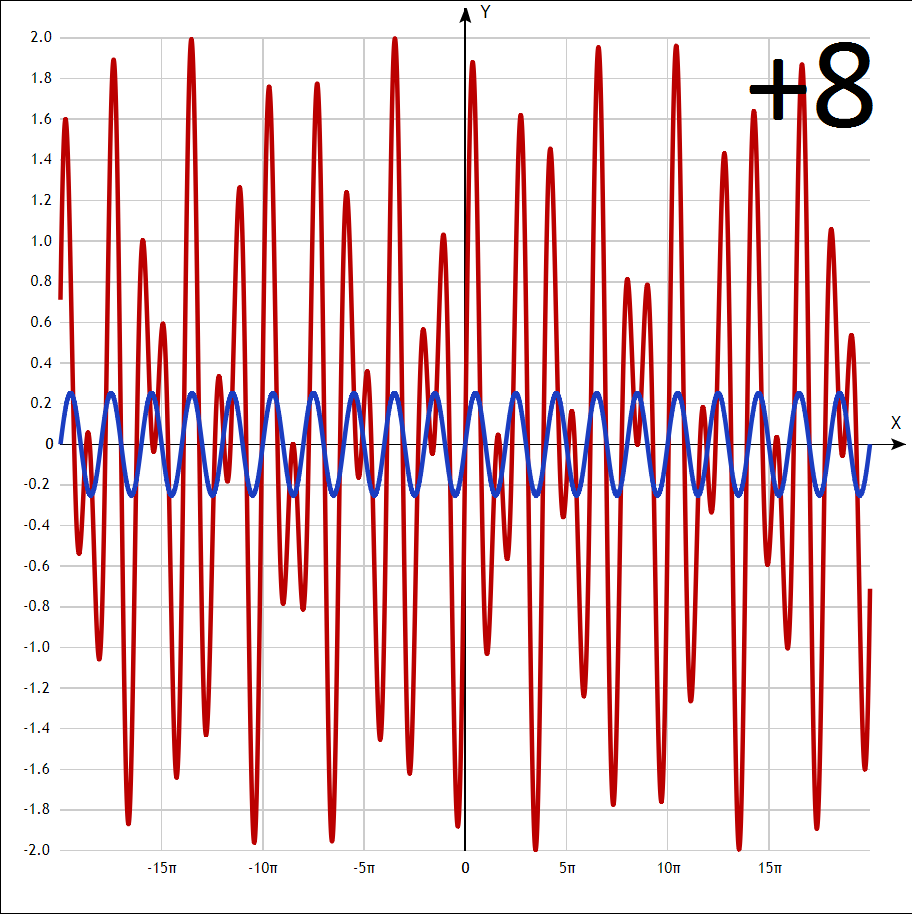
\includegraphics[width=0.45\textwidth]{fig/intervals/i08}
            & 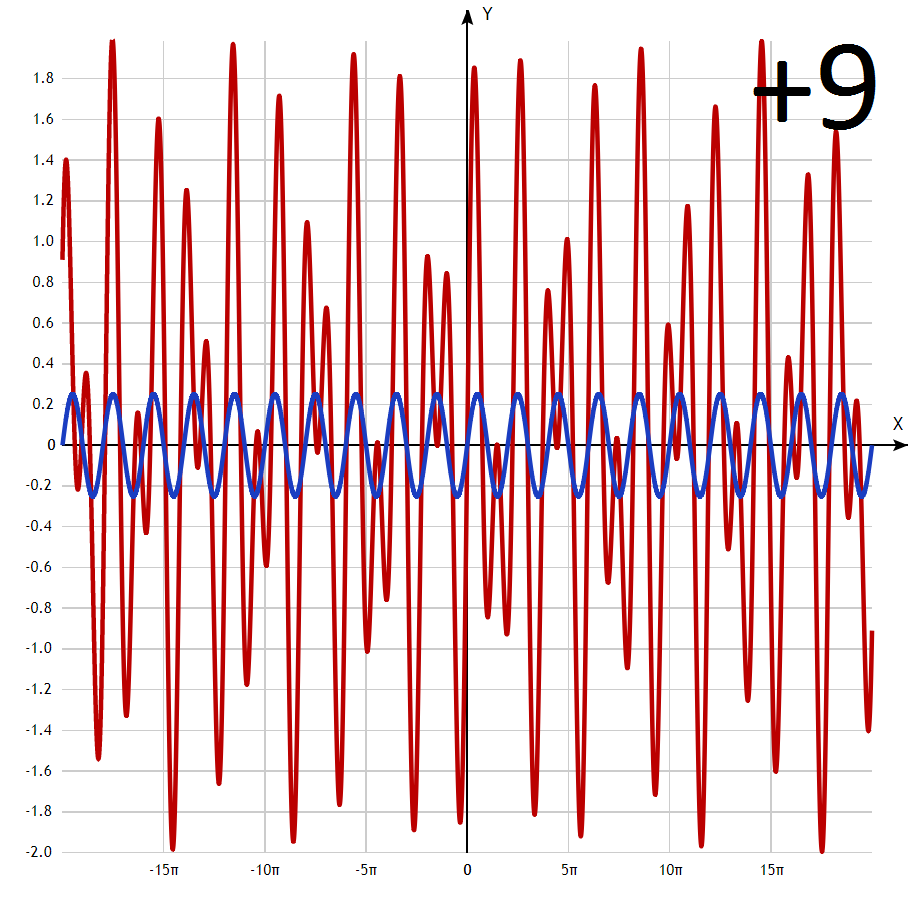
\includegraphics[width=0.45\textwidth]{fig/intervals/i09} \\
        \hline\hline
    \end{tabular}
\end{table}

\begin{table}[!ht]
    \caption{Совершенные консонансы в графиках функции \eqref{eq:harmony:interval:sin}}
    \label{t:harmony:interval:conso-5-7}
    \centering
    \begin{tabular}{c|c}
        \hline\hline
        5 полутонов, $n=5$  & 7 полутонов, $n=7$ \\
        чистая кварта       & чистая квинта \\
        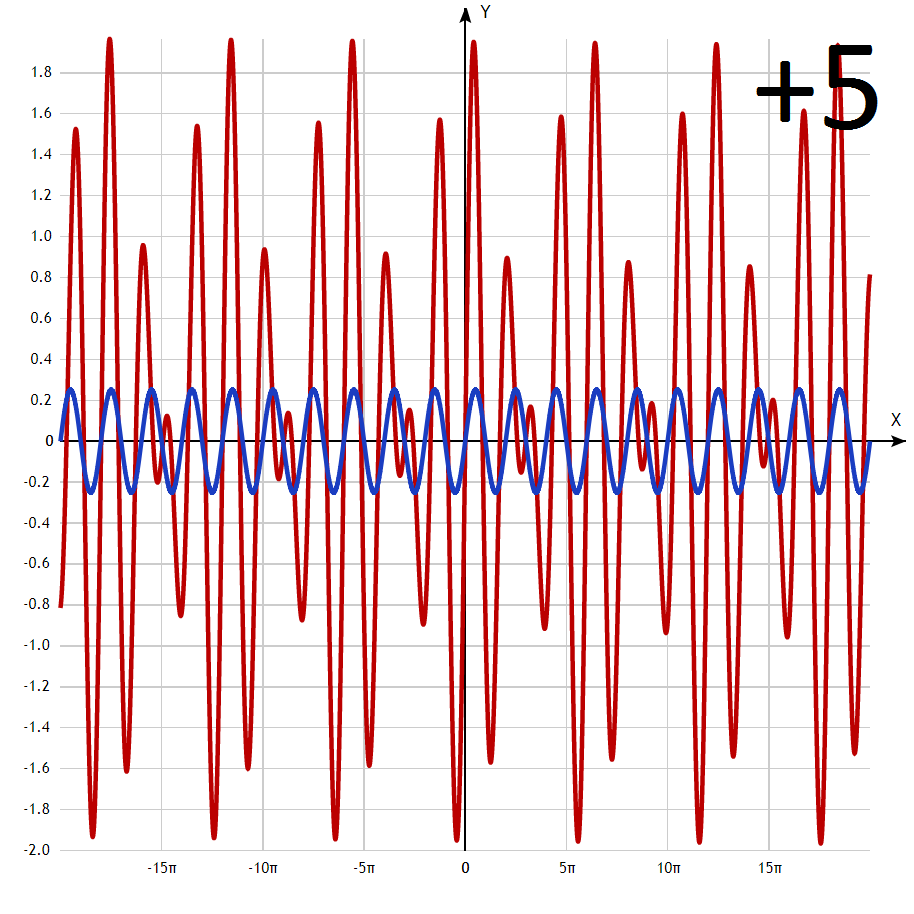
\includegraphics[width=0.45\textwidth]{fig/intervals/i05} 
            & 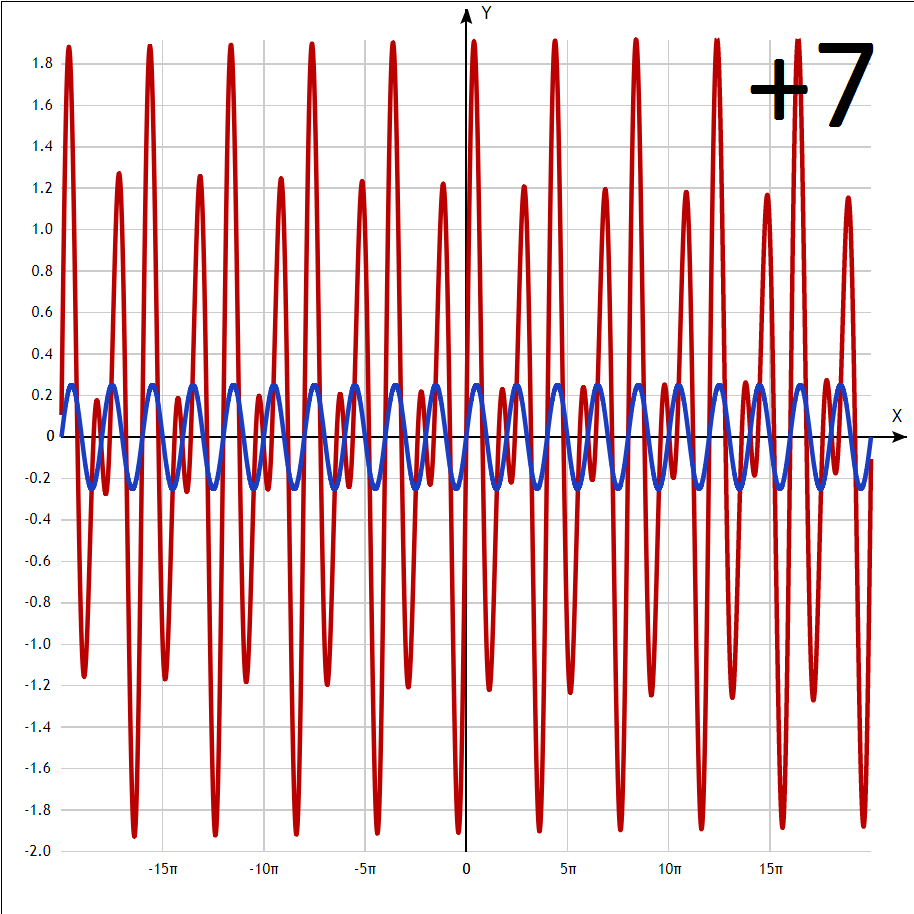
\includegraphics[width=0.45\textwidth]{fig/intervals/i07} \\
        \hline\hline
    \end{tabular}
\end{table}

\begin{table}[!ht]
    \caption{Диссонанс в графике функции \eqref{eq:harmony:interval:sin}}
    \label{t:harmony:interval:disso-6}
    \centering
    \begin{tabular}{c}
        \hline\hline
        6 полутонов, $n=6$ \\
        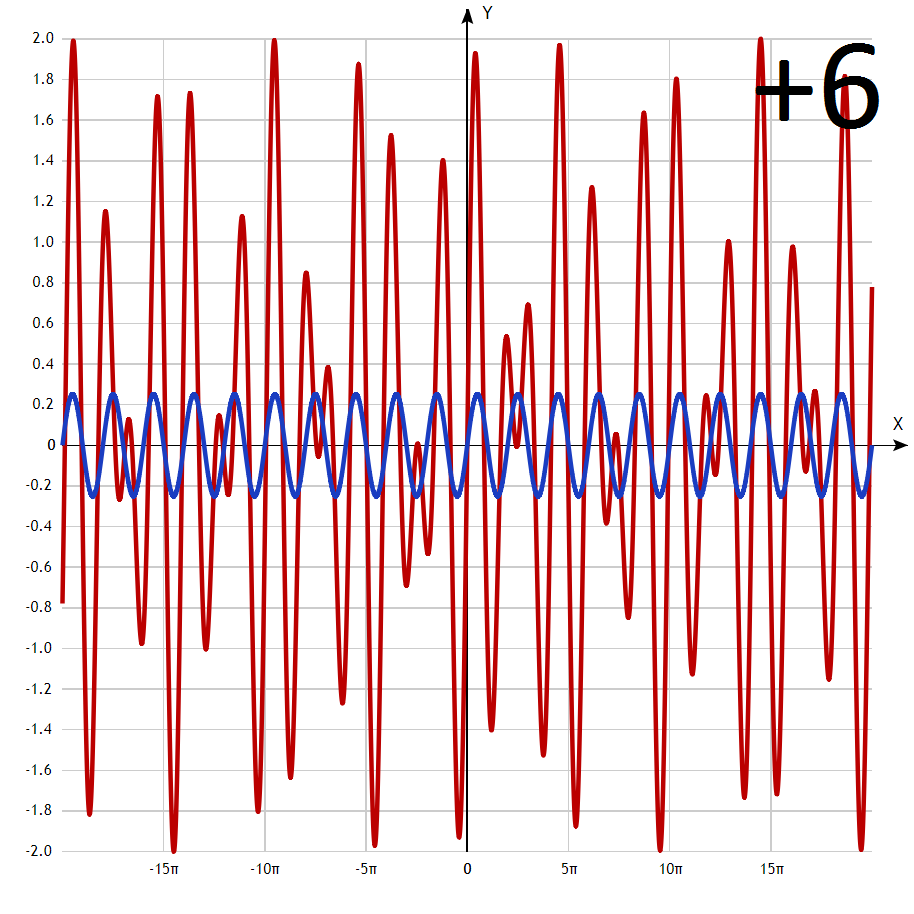
\includegraphics[width=0.45\textwidth]{fig/intervals/i06} \\
        увеличенная кварта,\\
        она же --- уменьшенная квинта,\\
        он же --- тритон\\
        \hline\hline
    \end{tabular}
\end{table}

Звуки октавы удобно зациклить и изобразить на окружности. На рисунке \ref{fig:harmony:interval:oct-round} изображены ноты октавы и отмечены консонансы и диссонансы от ноты ДО (т.е. C --- ноты обозначены в латинской нотации). Кстати, можно сделать удобный приборчик для определения консонансов и диссонансов, если сделать кружок с нотами подвижным. Но погодите. Если уж делать, то квинто-квартовый круг (см. раздел \ref{ch:harmony:kvinto-kvarto-round}).

\begin{figure}[!ht]
    \centering
    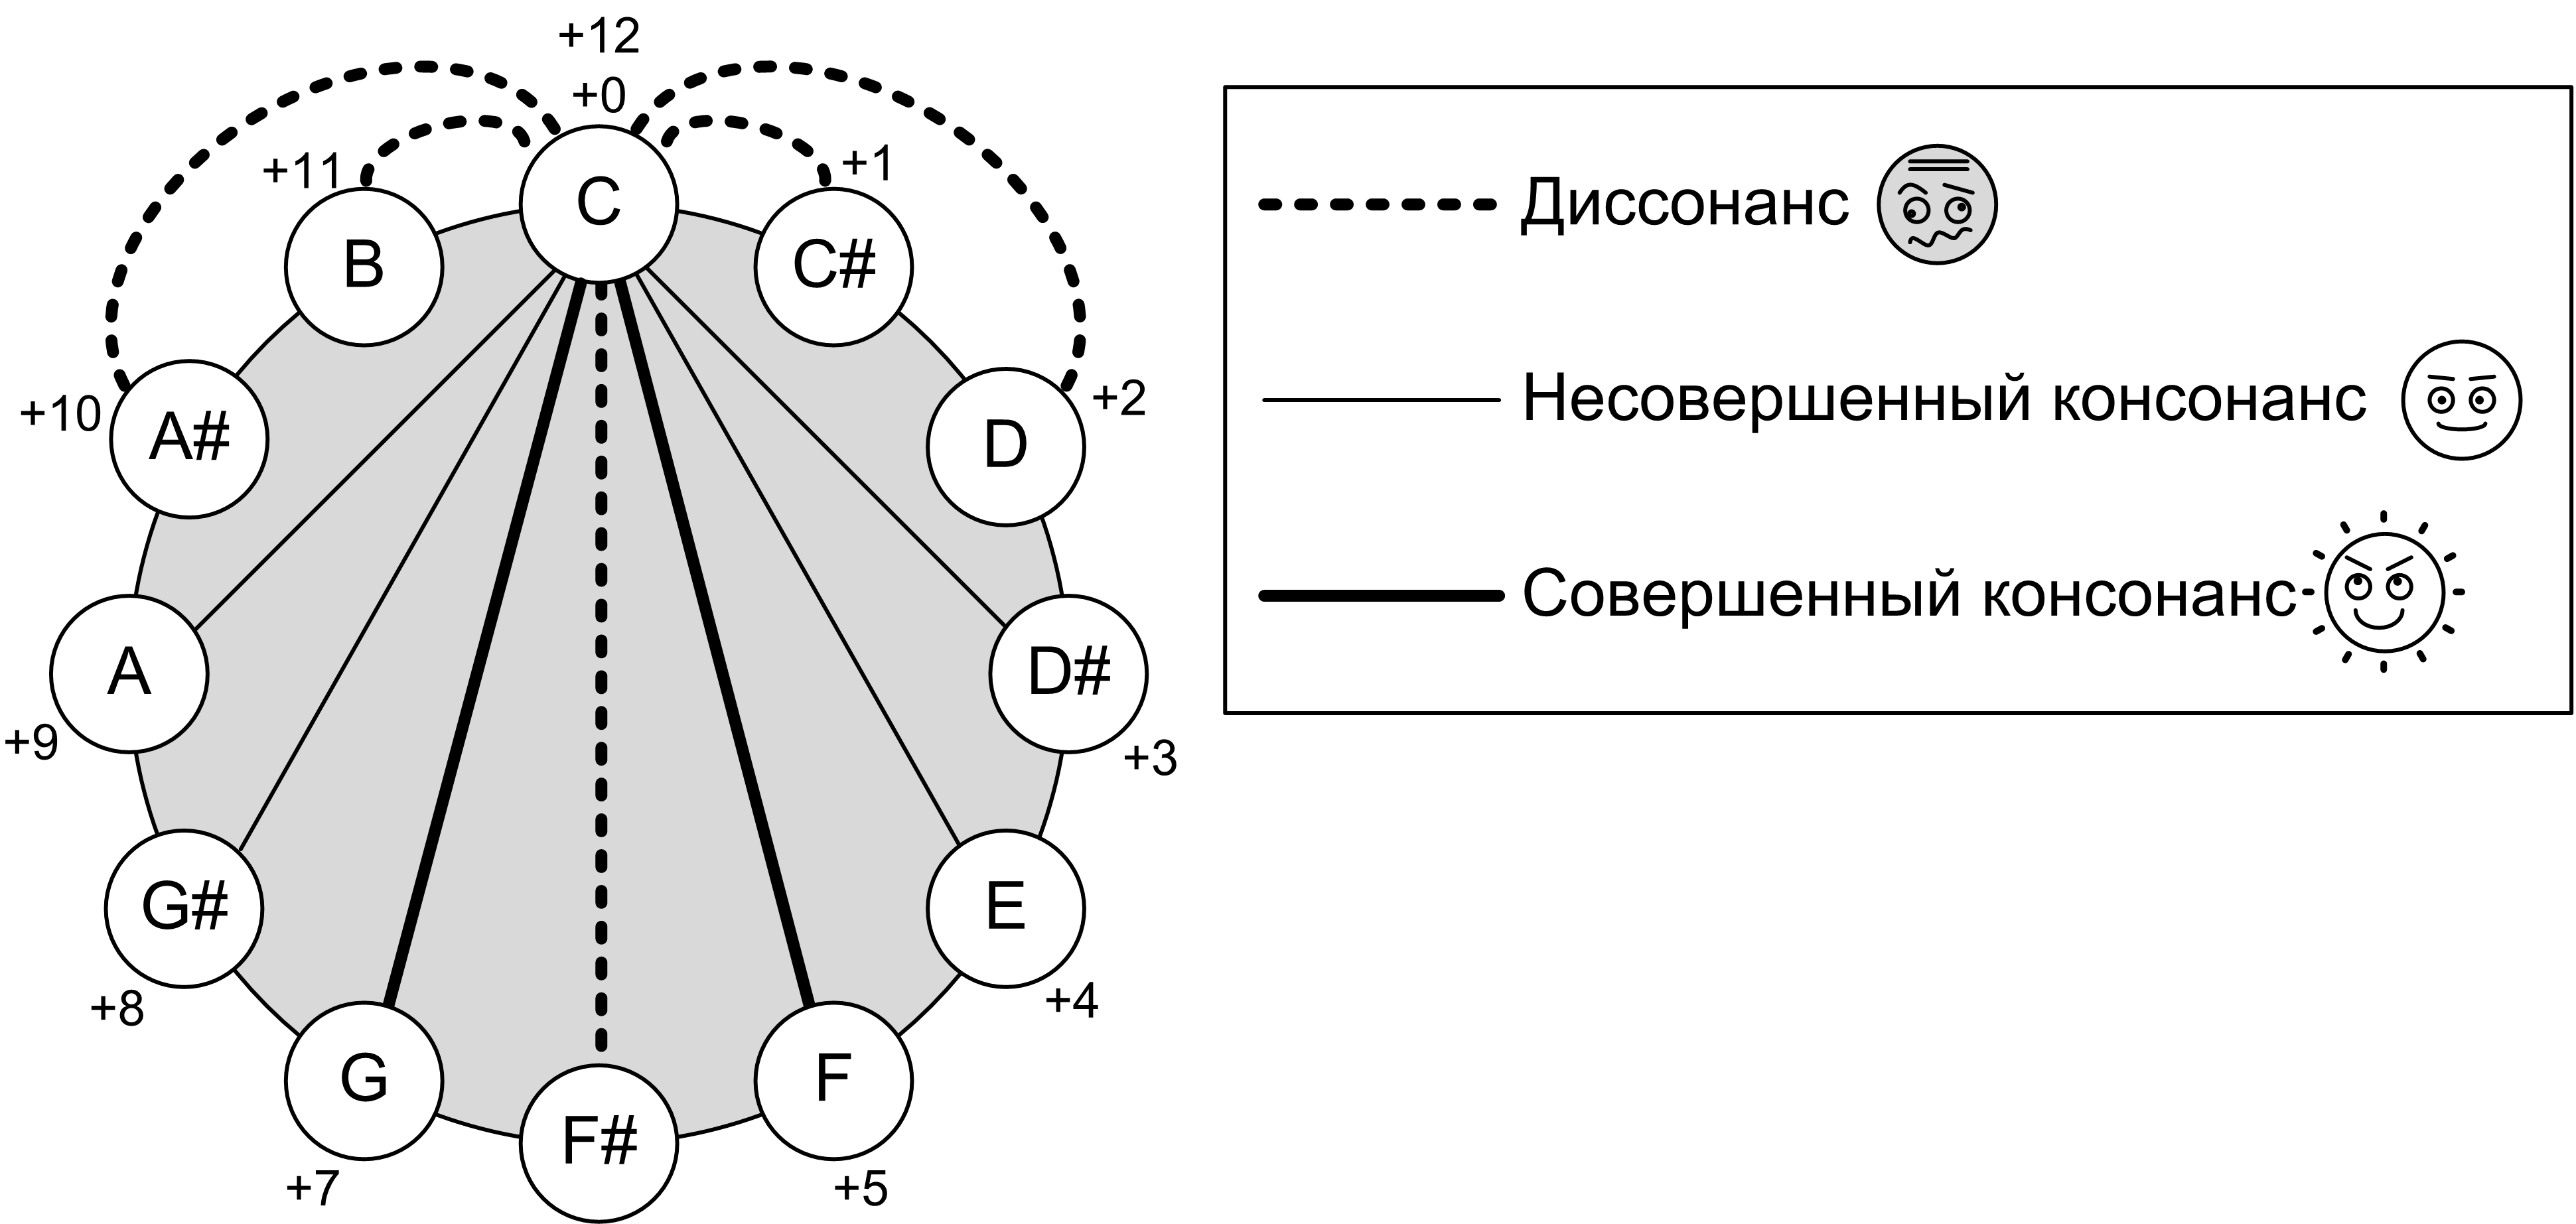
\includegraphics{fig/intervals/octave-round} 
    \caption{Интервалы от ноты ДО}\label{fig:harmony:interval:oct-round}
\end{figure} 

Осталось разобраться какого лешего интервалы называются так странно? Нет никакой видимой связи между названиями интервала и количеством полутонов, его составляющих! Справочник\footnote{Для тех, кому зубрежка покажется проще понимания} по интервалам см. в таблице \ref{t:harmony:interval:names}. Собственно, ответ прост: по историческим причинам название интервала отражало не количество полутонов, а номер ступени мажорного музыкального лада (о ладах см. раздел \ref{ch:harmony:lad}). Так как каждая ступенька мажорного лада состояла из одного или двух полутонов, то определить количество полутонов по названию интервала без достаточного опыта затруднительно, если не представить в уме рисунок \ref{fig:harmony:interval:names}.

\begin{table}[!ht]
    \caption{Интервалы}
    \label{t:harmony:interval:names}
    \centering
    \begin{tabular}{l|l|l|c|l}
        \hline\hline
        Название интервала & Перевод            &               & Количество  & Кратко  \\
                           & на русский         &               & полутонов   &         \\
        \hline\hline
        Прима(prima)       & Первая (ступень)   & Чистая        & 0                 & ч.1 \\
        Секунда(secunda)   & Вторая             & Малая         & 1                 & м.2 \\
                           &                    & Большая       & 2                 & б.2 \\
        Терция(tertia)     & Третья             & Малая         & 3                 & м.3 \\
                           &                    & Большая       & 4                 & б.3 \\
        Кварта(quarta)     & Четвертая          & Чистая        & 5                 & ч.4 \\
                           &                    & Увеличенная   & 6                 & ув.4\\
        Квинта(quinta)     & Пятая              & Уменьшенная   & 6                 & ум.5\\
                           &                    & Чистая        & 7                 & ч.5 \\
        Секста(sexta)      & Шестая             & Малая         & 8                 & м.6 \\
                           &                    & Большая       & 9                 & б.6 \\
        Септима(septima)   & Седьмая            & Малая         & 10                & м.7 \\
                           &                    & Большая       & 11                & б.7 \\
        Октава(octava)     & Восьмая            & Чистая        & 12                & ч.8 \\
        \hline\hline
        Нона(nona)         & Девятая            & Малая         & 13                & м.9  \\
                           &                    & Большая       & 14                & б.9  \\
        Децима(decima)     & Десятая            & Малая         & 15                & м.10 \\
                           &                    & Большая       & 16                & б.10 \\
        Ундецима           & Одиннадцатая       & Чистая        & 17                & ч.11 \\
                           &                    & Увеличенная   & 18                & ув.11\\
        Дуодецима          & Двенадцатая        & Уменьшенная   & 18                & ум.12\\
                           &                    & Чистая        & 19                & ч.12 \\
        Терцдецима         & Тринадцатая        & Малая         & 20                & м.13 \\
                           &                    & Большая       & 21                & б.13 \\
        Квартдецима        & Четырнадцатая      & Малая         & 22                & м.14 \\
                           &                    & Большая       & 23                & б.14 \\
        Квинтдецима        & Пятнадцатая        & Чистая        & 24                & ч.15 \\
        \hline\hline
    \end{tabular}
\end{table}

\begin{figure}[!ht]
    \centering
    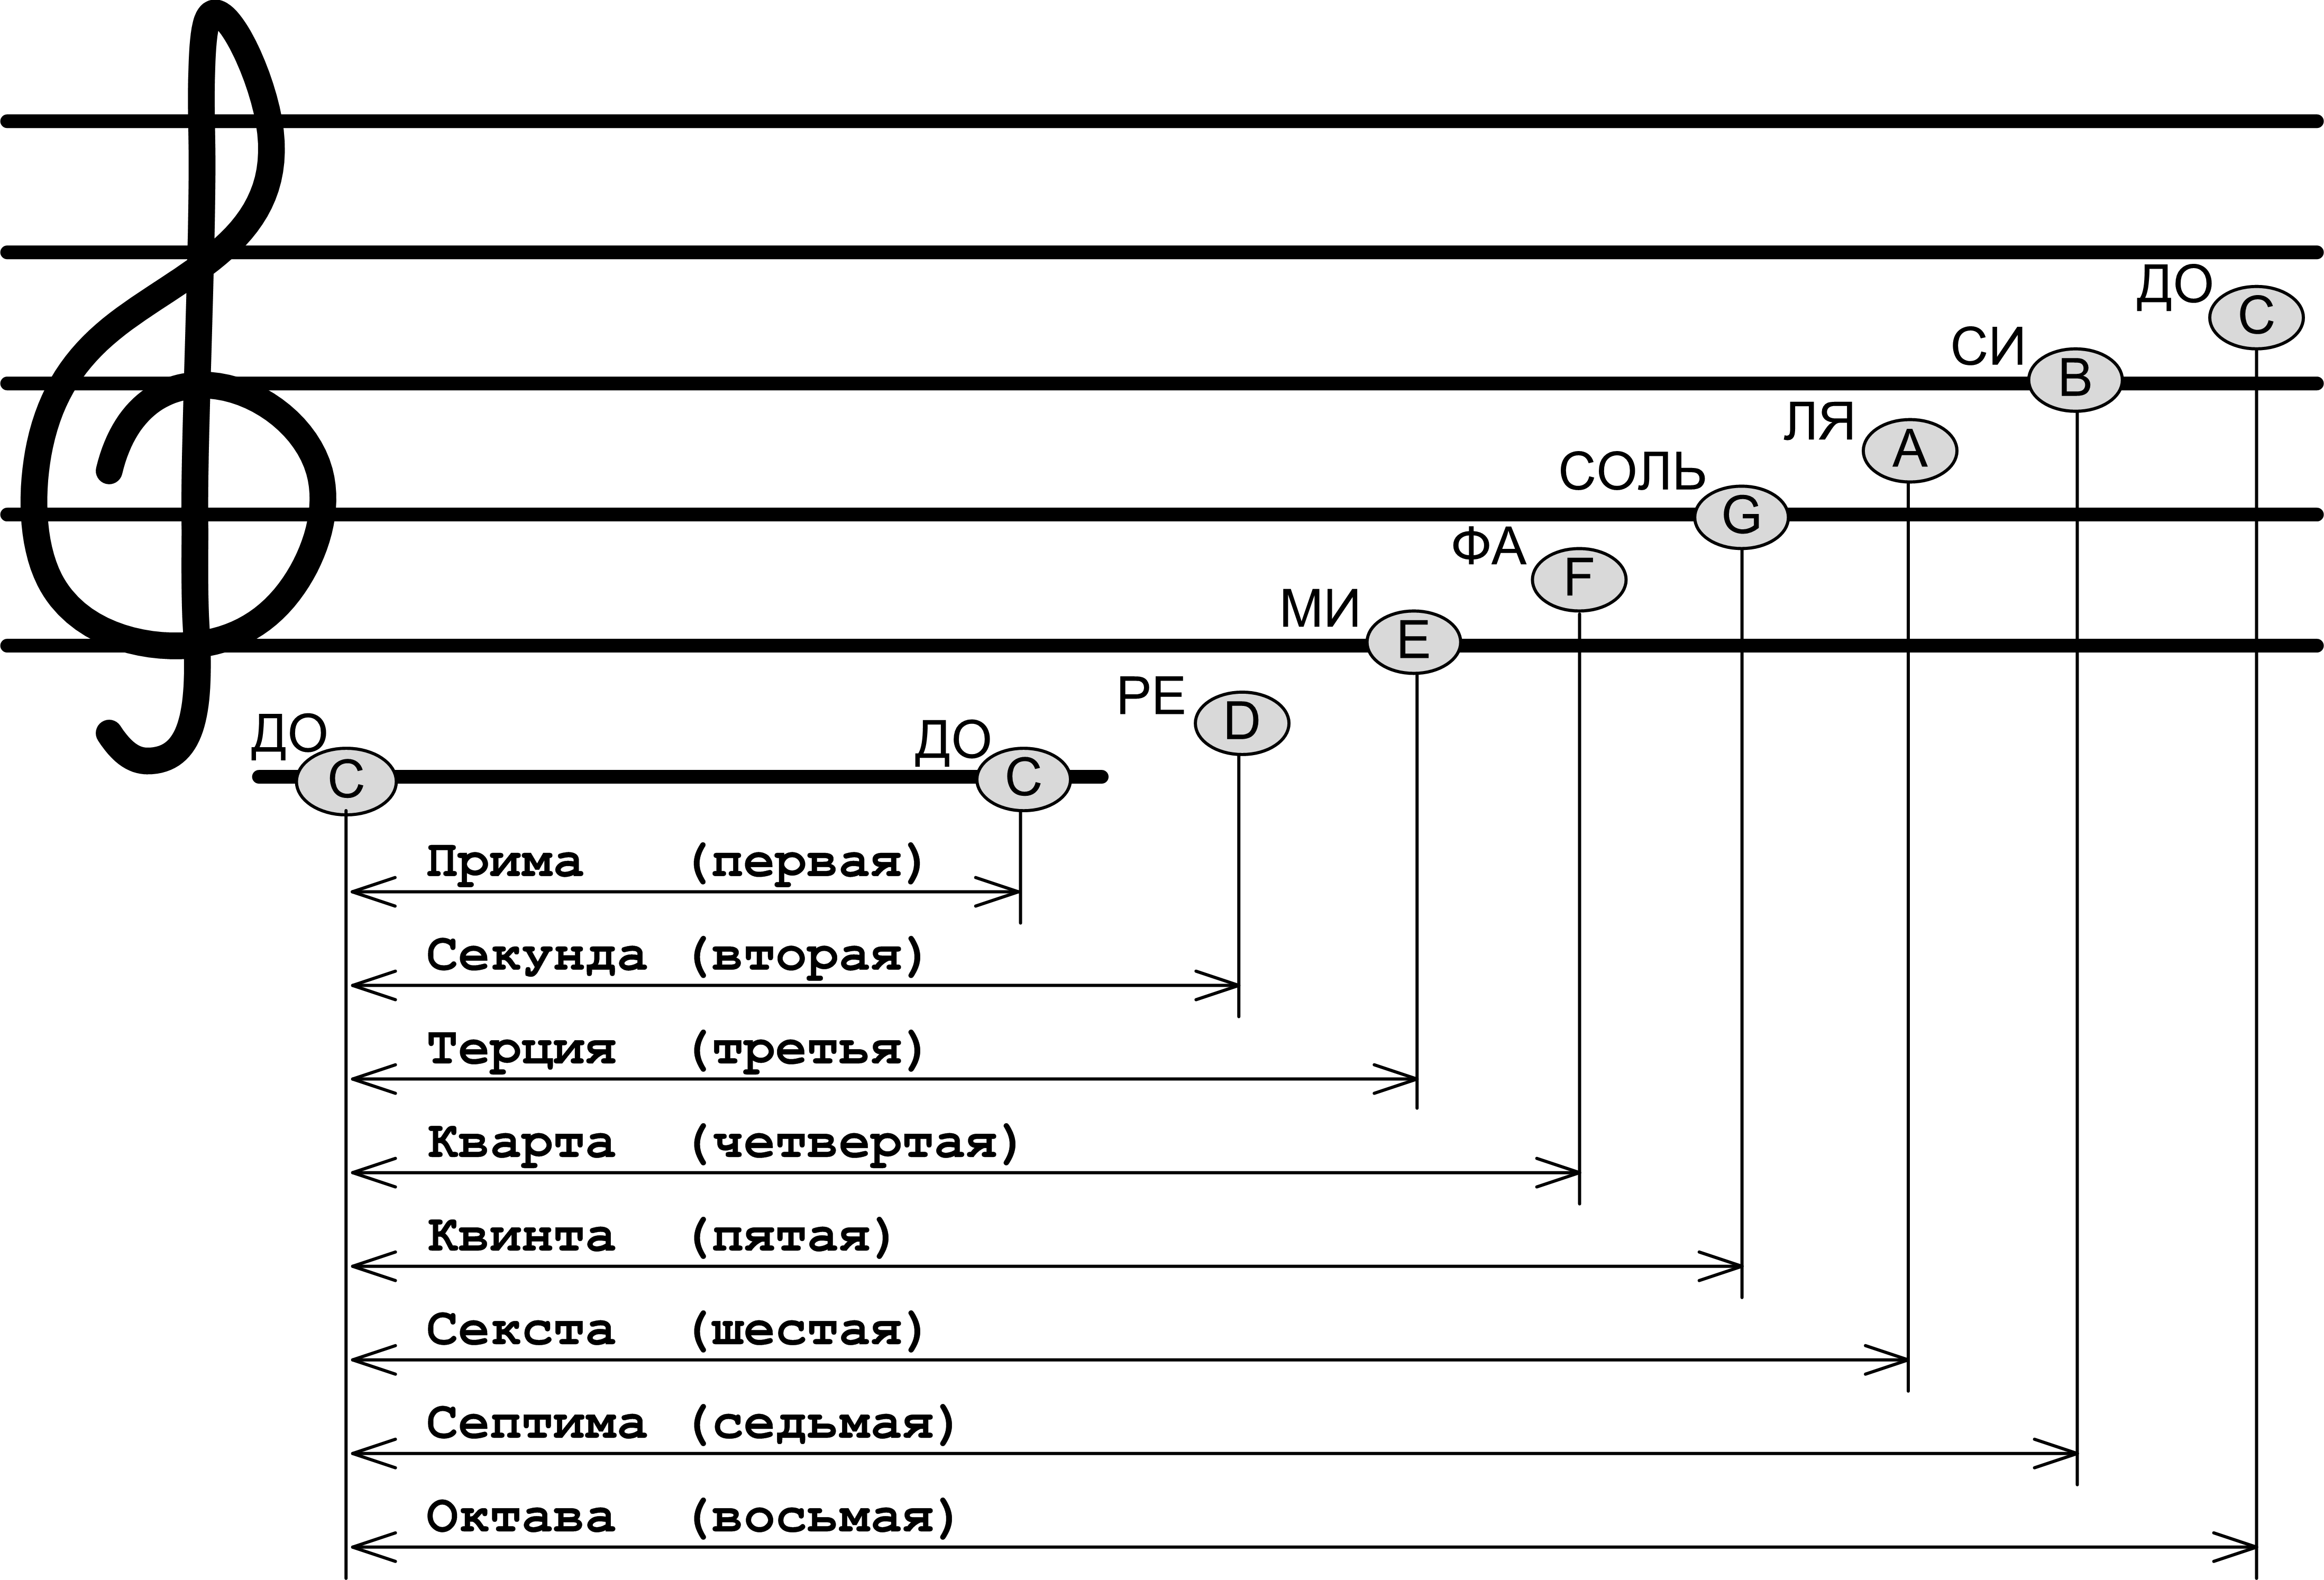
\includegraphics{fig/intervals/interval-names} 
    \caption{Исторически имена интервалов --- это имена ступеней мажорного лада}\label{fig:harmony:interval:names}
\end{figure} 

Тогда все становится относительно просто. Например, терция, это расстояние от ноты ДО (первая ступень мажорного лада) до ноты МИ (третья ступень). Считаем ДО-РЕ --- 2 полутона, РЕ-МИ --- 2-а полутона. Получилось 4-е полутона. Только вот вспоминается, что терция бывает <<большая>> и <<малая>>. При таком подходе мы всегда будем получать значение для <<большого>> и <<чистого>> интервалов. Для <<малого>> или <<уменьшенного>> интервалов нужно уменьшить получившееся число на 1, а для <<увеличенного>> --- увеличить на 1. Значит: большая терция --- 4 полутона, малая --- 3.

Закрепим. Например, квинта: расстояние ДО-СОЛЬ --- 7 полутонов. Уменьшенная квинта --- 6 полутонов, чистая --- 7.


\section{Лады? Лады}
\label{ch:harmony:lad}

\begin{Definition}[Лад]
    \emph{Лад}\footnote{В переводе на английский: Mode} --- это интервальный шаблон, позволяющий из 12-и последовательных музыкальных звуков октавы выбрать \emph{условно} <<правильные>>. 
\end{Definition}

Если это определение показалось вам тяжеловатым, почитайте учебники или Википедию. От некоторых определений веет такой суровой философией, что хочется курить в глубокий затяг. 

Задача лада: из 12 музыкальных звуков, составляющих октаву, выбрать лишь несколько таких, которые можно играть в любом порядке и все равно будет МУЗЫКА! Задача не из тривиальных и кажется весьма субъективной, ведь всегда найдется кто-то, кто скажет: <<А мне не нравится!>>. 

Однако эта задача была решена\footnote{Не исключено, что кем-то она решается и в данный момент} предками неоднократно, и в культурном наследнии мы имеем немало ладов, самыми известными из которых являются \emph{мажорный} и \emph{минорный}.

Мажорный и минорный лады --- лады семиступенные. То есть такой лад выбирает из 12 звуков октавы только 7.


\paragraph{Мажорный лад}

Начнем с мажорного лада, интервальная структура которого приведена на рисунке \ref{fig:harmony:lad:mode:maj}. Тёмными кружками обозначены <<выбранные>> ладом звуки --- \emph{ступени} лада. Например, вторая ступень мажорного лада находится на расстоянии 2-х полутонов от первой. Интервалы (в полутонах) между ступенями \emph{мажорного} лада расположены так:

\[
    \texttt{2-2-1-2-2-2-1}
\]

Всем с детства знакомое ДО, РЕ, МИ, ФА, СОЛЬ, ЛЯ, СИ есть не что иное, как 7 идеальных ноток, отобранных мажорным ладом, начиная от ноты ДО. Проверьте: (ДО-РЕ)=2 полутона, (РЕ-МИ)=2, (МИ-ФА)=1, (ФА-СОЛЬ)=2 и т.д. 

Интересно то, что уникальные имена получили только 7 нот, а остальные 5 нот октавы имеют производные имена (с суффиксом <<бемоль>> или <<диез>>) --- есть следствие использования ладов.

\begin{figure}[!ht]
    \centering
    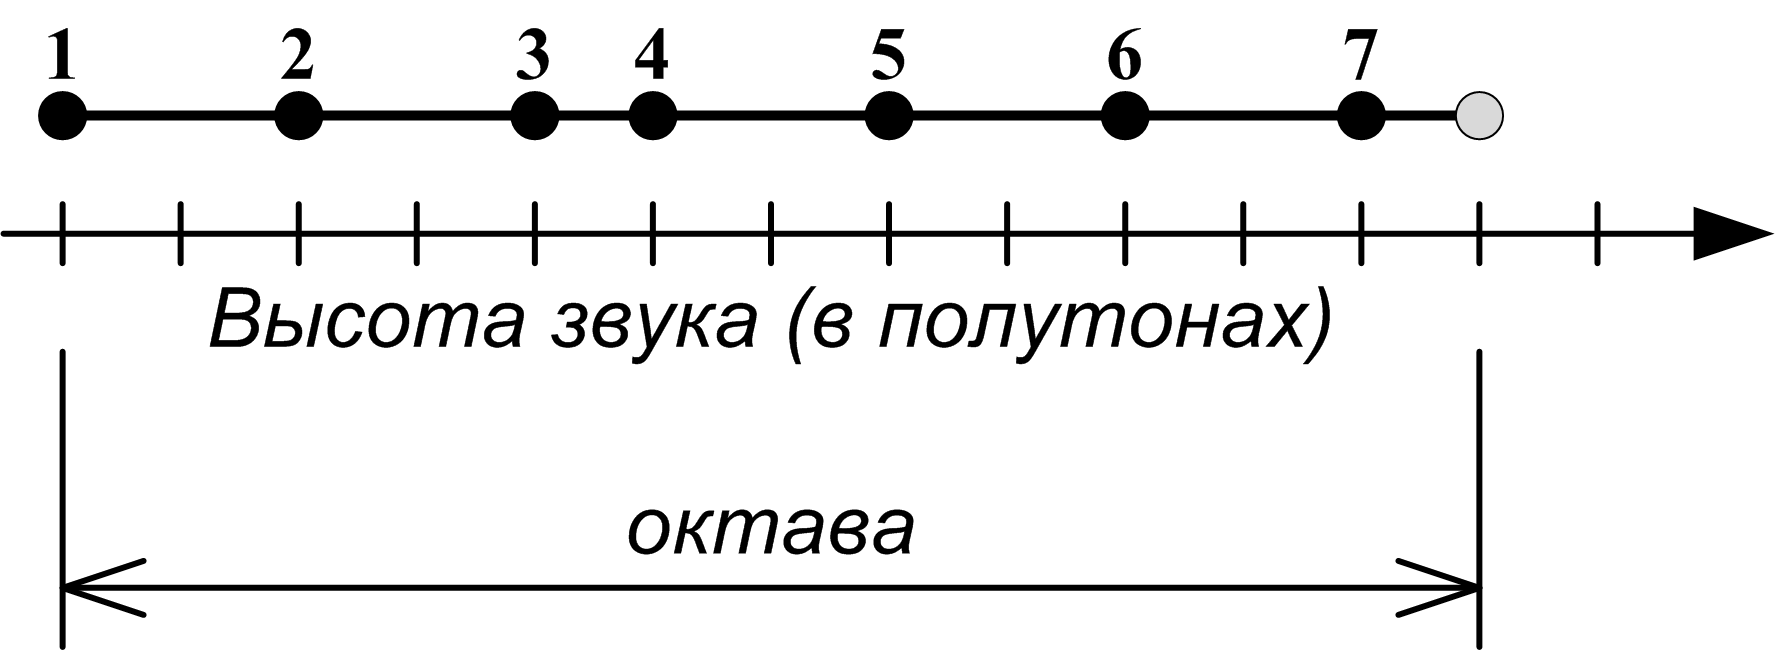
\includegraphics{fig/intervals/mode-maj} 
    \caption{Интервальная структура мажорного лада}\label{fig:harmony:lad:mode:maj}
\end{figure} 

Таким образом, шаблон лада может накладываться на любую ноту, любой музыкальный звук. Сплошная теория относительности!

Когда первая ступень лада накладывается на определенную ноту, то набор нот, попавших на ступени лада, образует \emph{тональность}. Допустим, мы совместили первую ступень мажорного лада с нотой ДО, тогда мы получим тональность <<ДО-мажор>>: ДО, РЕ, МИ, ФА, СОЛЬ, ЛЯ, СИ. Название тональности складывается из названия ноты, попавшей на первую ступень и названия лада. Обычно мелодия составляется только из семи нот, входящих в тональность. Так и говорят, например, мелодия в тональности <<ЛЯ-минор>>.

\begin{Example}[Тональность <<РЕ-мажор>>]
    \label{ex:harmony:lad:d:maj}
    
    Чтобы получить ноты в тональности РЕ-мажор, нам нужно совместить ноту РЕ и первую ступень мажорного лада. Отступаем два полутона, и на вторую ступень попадет нота МИ. На третью --- ФА-диез.
    
    Целиком:
    \begin{center}
        РЕ, МИ, ФА-диез, СОЛЬ, ЛЯ, СИ, ДО-диез.
    \end{center}
\end{Example}

Чтобы сыграть \emph{гамму} в заданной тональности нужно:
\begin{itemize}
    \item начать с ноты первой ступени;
    \item продолжить играть ноты тональности в порядке возрастания (или убывания) высоты;
    \item сыграв таким образом одну или несколько октав, закончить на ноте первой ступени (естественно уже в другой октаве); 
    \item (необязательно) проиграть только что сыгранную последовательность в обратном порядке.
\end{itemize}

Например, гамма в тональности <<ДО-мажор>> или просто <<гамма ДО-мажор>> это известное: 
\begin{center}
    ДО, РЕ, МИ, ФА, СОЛЬ, ЛЯ, СИ, ДО, СИ, ЛЯ, СОЛЬ, ФА, МИ, РЕ, ДО.
\end{center}


\paragraph{Минорный лад}

Интервальная структура \emph{минорного} лада приведена на рисунке \ref{fig:harmony:lad:mode:min}. Интервалы (в полутонах) между ступенями \emph{минорного} лада расположены так:
\[
    \texttt{2-1-2-2-1-2-2}
\]

\begin{figure}[!ht]
    \centering
    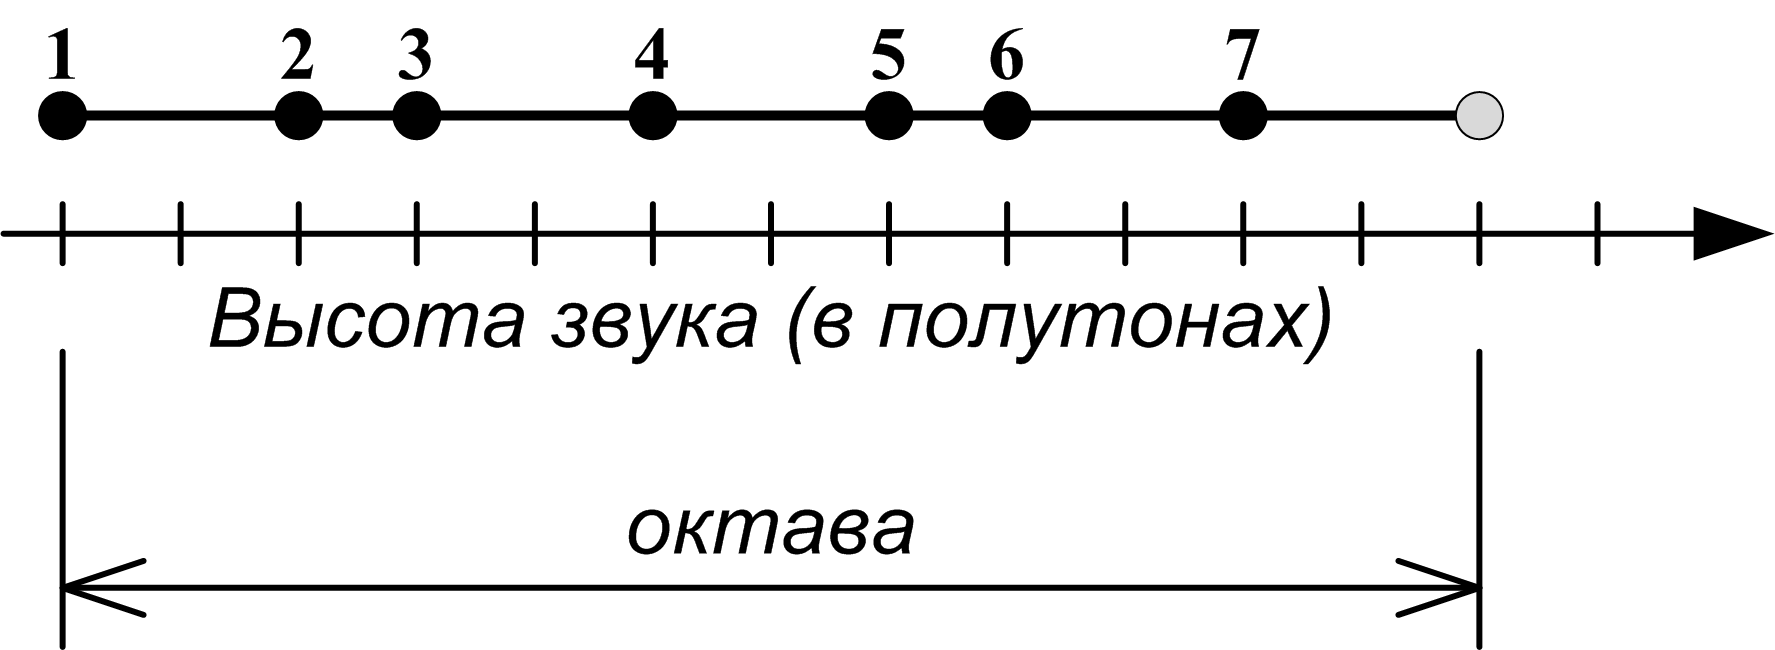
\includegraphics{fig/intervals/mode-min} 
    \caption{Интервальная структура минорного лада}\label{fig:harmony:lad:mode:min}
\end{figure} 

Заметьте, что если замкнуть минорную интервальную структуру в кольцо и немного повращать (а это можно сделать, так как в следующей октаве все повторится), то получится мажорный лад. Совместите первую ступень мажорного лада и третью минорного и убедитесь, что в принципе структура этих ладов одна и та же. 

Например, давайте положим в первую ступень минора ноту ЛЯ. Получим тональность, состоящую из нот:
\begin{center}
    ЛЯ, СИ, ДО, РЕ, МИ, ФА, СОЛЬ.
\end{center}

Ноты в тональности <<ЛЯ-минор>> те же, что и в <<ДО-мажор>> (как видно ни одной нотки с бемолем или диезом). Поэтому тональности <<ДО-мажор>> и <<ЛЯ-минор>> называются \emph{параллельными}. Как нетрудно догадаться, параллельных тональностей столько же, сколько фактических нот в октаве: 12. А вот гамму <<ЛЯ-минор>>:
\begin{center}
    ЛЯ, СИ, ДО, РЕ, МИ, ФА, СОЛЬ, ЛЯ, СОЛЬ, ФА, МИ, РЕ, ДО, СИ, ЛЯ
\end{center}
с гаммой <<ДО-мажор>> точно на слух не спутаешь!






\section{Чем больше, тем лучше? Аккорды}
\label{ch:harmony:chords}

TODO

\section{Так квинтовый или квартовый? Квинто-квартовый круг}
\label{ch:harmony:kvinto-kvarto-round}

Замечателен тот факт (см. рисунок \ref{fig:harmony:interval:oct-round}), что для отдельно взятого звука в пределах октавы можно подобрать лишь \emph{два} звука, образующий с исходным звуком совершенный консонанс. Можно ли переупорядочить ноты на рисунке \ref{fig:harmony:interval:oct-round} так, чтобы звуки, образующие с исходным звуком совершенный консонанс, стали его (исходного звука) соседями: один справа, другой слева?

Можно, иначе быть не может! Давайте выпишем последовательность идущих друг за другом совершенных консонансов, отступая всякий раз кварту (5 полутонов). Начнем с ноты C. Кварта вверх от C --- это G. Кварта вверх от G --- D. И так далее. В результате получим:
\begin{center}
    C, G, D, A, E, B, 
\end{center}